% !TEX root = developer.tex


\chapter{Hardware Models}
\label{chapter:hardware}

\section{Overview}
\label{sec:topOverview}
To better understand how hardware models are put together for simulating interconnects, we should try to understand the basic flow of event in SST/macro involved in sending a message between two network endpoints.  We have already seen in skeleton applications in previous sections how an application-level call to a function like \inlinecode{MPI_Send} is mapping to an operating system function and finally a hardware-level injection of the message flow.  Overall, the following steps are required:

\begin{itemize}
\item Start message flow with app-level function call
\item Push message onto NIC for send
\item NIC packetizes message and pushes packets on injection switch
\item Packets are routed and traverse the network
\item Packets arrive at destination NIC and are reassembled (potentially out-of-order)
\item Message flow is pushed up network software stack
\end{itemize}

Through the network, packets must move through buffers (waiting for credits) and arbitrate for bandwidth through the switch crossbar and then through the ser/des link on the switch output buffers.  The control-flow diagram for transporting a flow from one endpoint to another via packets is shown in Figure \ref{fig:controlFlow}

In general, sending data across the network (as in, e.g.., MPI), requires the following components:

\begin{itemize}
\item Packetization: handled by \inlinecode{nic} class. Converts flows (MPI messages) into smaller packets.
\item Network topology: handled by \inlinecode{topology} class. Defines the geometry of the network, determining how nodes are connected to switches and how switches are interconnected. It also defines which ports are used for each connection.
\item Fabric management (not yet implemented in SST)
\item Routing: handled by \inlinecode{router} class. Using the defined topology, compute the path that should be taken by a packet. The path is defined by the port numbers that should be taken.
\item Flow control and congestion: handled by \inlinecode{NetworkSwitch} class. Once a path is defined by the router, arbitrate packets (flits) when they contend for bandwidth.
\end{itemize}
As much as possible, these components try to be independent. However, there are inter-dependencies, as shown in Figure \ref{fig:dependencies}.
The router requires topology information to compute paths. For adaptive routing decisions, the router also requires contention information from the network switch.
The network switch requires the computed paths (ports) from the router.

\begin{figure}
\centering
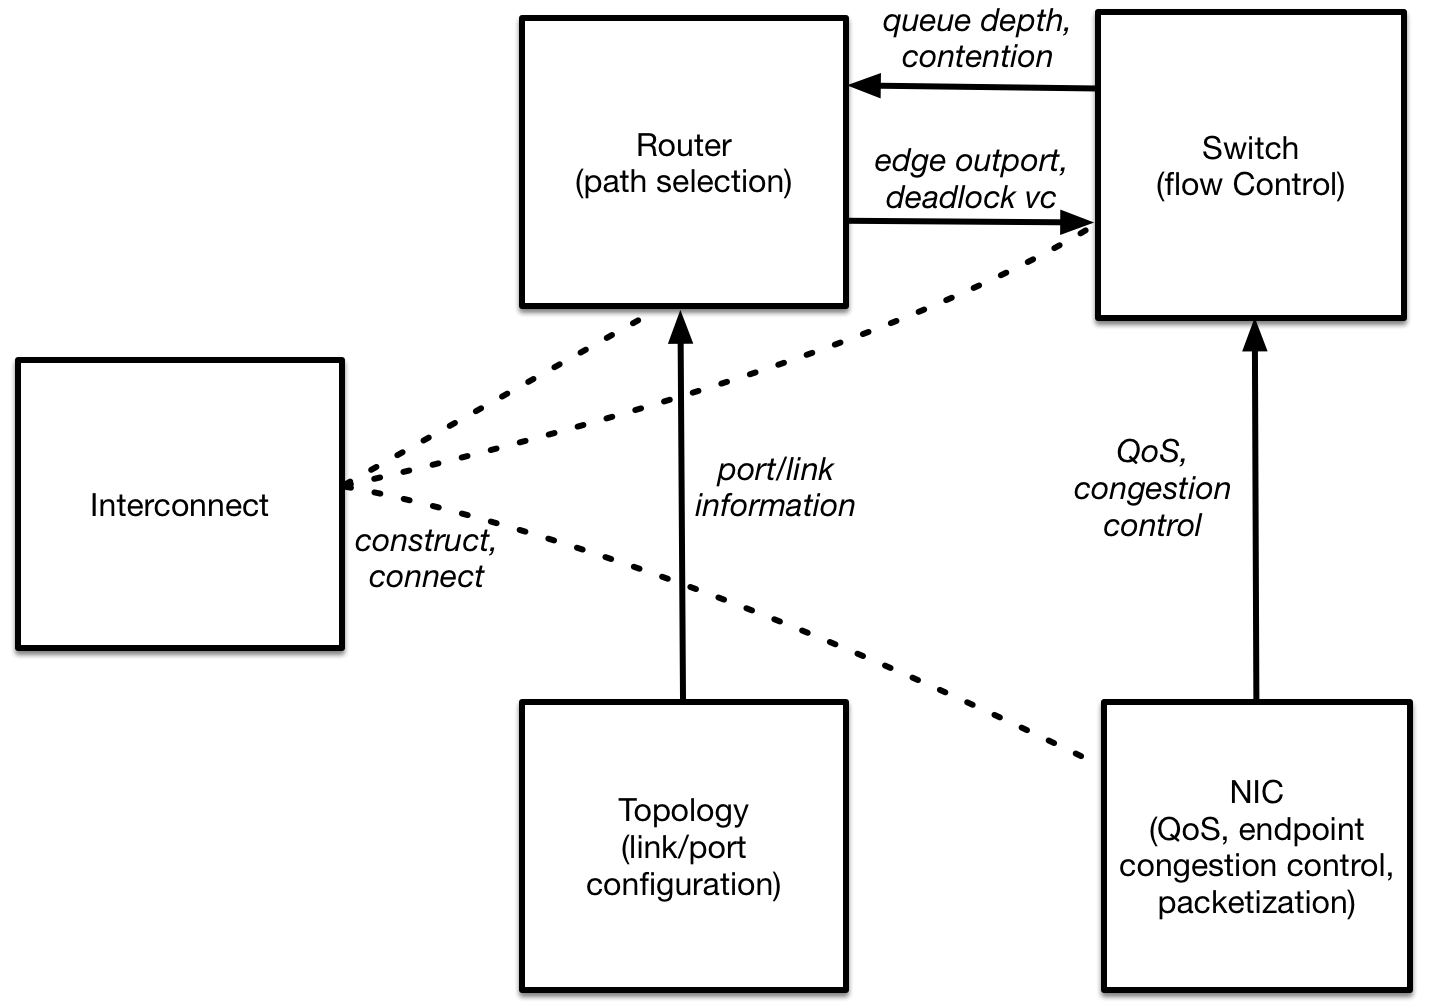
\includegraphics[width=1.0\textwidth]{figures/components}
\caption{Components used modeling interconnect and dependencies between them.}
\label{fig:dependencies}
\end{figure}

\begin{figure}
\centering
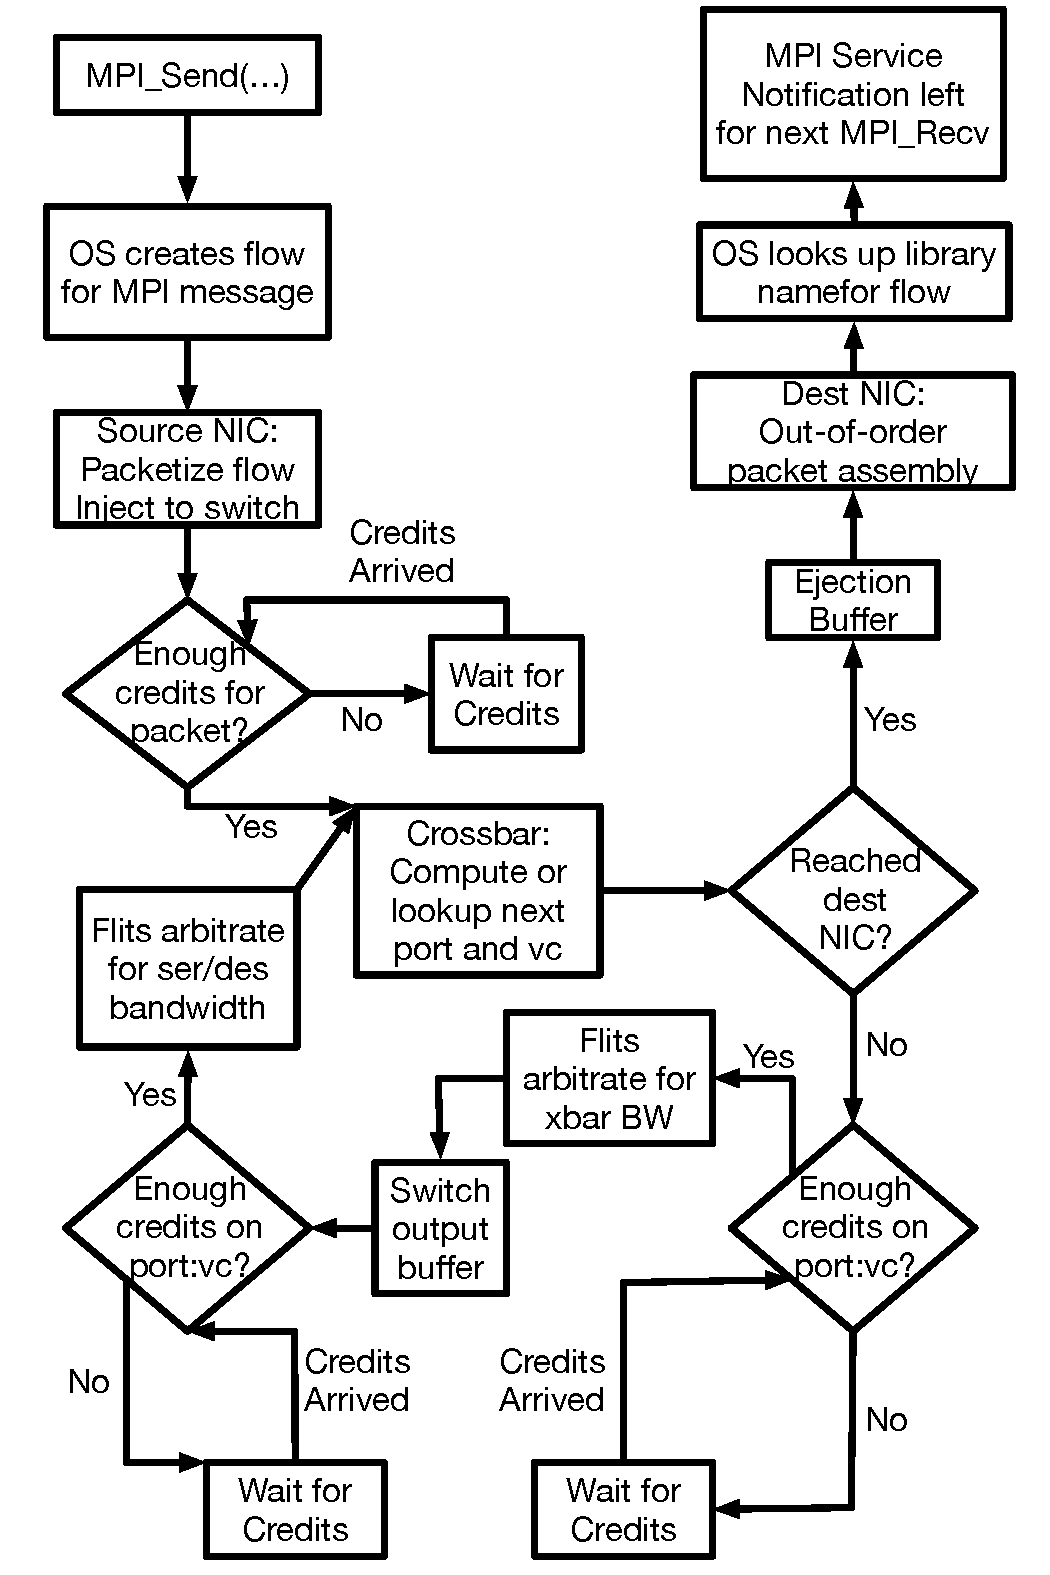
\includegraphics[width=0.75\textwidth]{figures/DecisionFlow}
\caption{Decision diagram showing the various control flow operations that occur as a message is transport across the network via individual packet operations.}
\label{fig:controlFlow}
\end{figure}

We can dive in deeper to the operations that occur on an individual component, mos importantly the crossbar on the network switch. Figure \ref{fig:xbarFlow} shows code and program flow for a packet arriving at a network switch.  The packet is routed (virtual function, configurable via input file parameters), credits are allocated to the packet, and finally the packet is arbitrated across the crossbar. After arbitration, a statistics callback can be invoked to collect any performance metrics of interest (congestion, traffic, idle time).

\begin{figure}
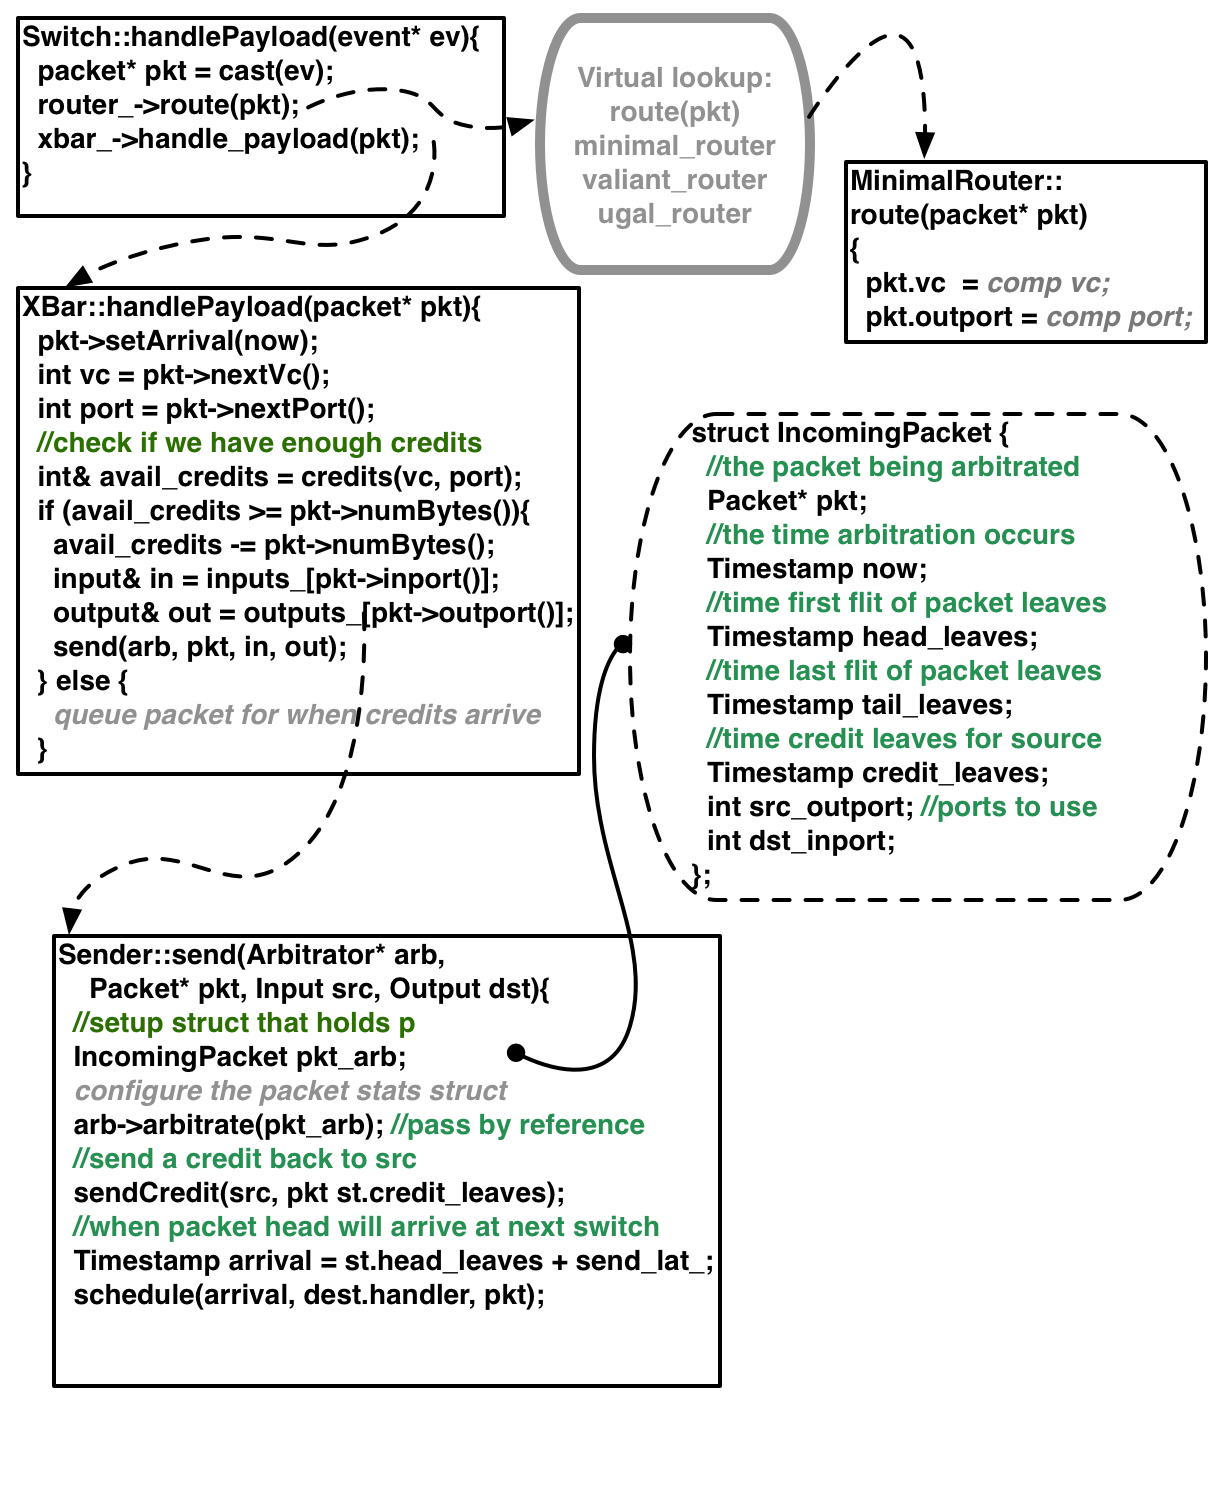
\includegraphics[width=0.9\textwidth]{figures/RoutingFlow}
\caption{Code flow for routing, arbitration, and stats collections of packets traversing the crossbar on the network switch.}
\label{fig:xbarFlow}
\end{figure}

\section{Packets}
Packet must hold information for endpoint control on the NIC, routing decisions, and flow control. 
Packets therefore suffer from a ``combinatorial explosion'' depending on which NIC model is coupled with which flow control mechanism and which routing algorithm.
For example, the simulator is intended to support at least two different network contention models (PISCES, SCULPIN);
five different topologies (torus, hyperX, fat tree, dragonfly, cascade); and four different routing algorithms (Minimal, Valiant, UGAL, PAR).
This creates already 40 combinations, which can grow even more quickly if new models are added.
If the C++ type of the packet were to depend on all of these, messy multiple inheritance patterns can result or 40 different packet types would be needed.
Some C++ patterns (e.g. policies) are designed to help implement combinatorial problems like this without multiple inheritance,
but this is not a good match for our case.

Flow control is generally the most complicated and requires the most data. 
\emph{Inheritance} from the base packet class is used to create packet types that are compatible with a particular congestion model.
For different routing or endpoint (NIC) methods, the packet object allocates blocks to be used as metadata for the different classes. 
These metadata blocks can then be cast as needed for each of the different functions.

\begin{CppCode}
char rtr_metadata_[MAX_HEADER_BYTES];
char nic_metadata_[MAX_NIC_BYTES];
\end{CppCode}
Defaults are chosen for the compile-time constants (8-16 bytes) and these can be changed as needed.
In the same way that a router or NIC allocates bits for certain functions, SST/macro uses bitsets stored in the metadata blocks.
For example, for adaptive routing on a dragonfly, we have the following bitset:

\begin{CppCode}
struct routing_header  {
 char is_tail : 1;
 uint16_t edge_port; 
 uint8_t deadlock_vc : 4;
 uint8_t num_group_hops : 2;
 uint8_t num_hops : 4;
 uint8_t stage_number : 3;
 uint32_t dest_switch : 24;
};
\end{CppCode}
The 54 bits here store the information needed by a router to implement progressive adaptive routing (PAR). 
For flow control on a particular type of switch, e.g. PISCES (see User's manual), we have a type \inlinecode{PiscesPacket}
that inherits from \inlinecode{packet} and adds the following fields:

\begin{CppCode}
class PiscesPacket : public packet {
....
uint8_t stage;
uint8_t outports[3];
uint16_t inport;
double bw_;
double max_in_bw_;
timestamp arrival_;
int current_vc_;
...
};
\end{CppCode}
These provide the path and flow control information needed to implement the PISCES contention model.

Inside router or switch flow control code, the metadata regions can be accessed as:
\begin{CppCode}
template <class T>
T* rtr_header()  {
  return (T*) (&rtr_metadata_);
}
\end{CppCode}
which returns the raw bytes cast to the correct C++ bitset type.

There is some universal information needed by all packets, which is not stored in the bitset:

\begin{CppCode}
NodeId toaddr_;
NodeId fromaddr_;
uint64_t flow_id_;
uint32_t num_bytes_;
serializable* payload_;
\end{CppCode}
This covers the source and destination nodes, a unique ID for the flow (e.g. MPI message) the packet came from, the number of bytes of the flow, and optionally a payload object carrying extra data.

To summarize, we have: \\

\begin{tabular}{lll}
\hline
Information & Where Stored & Access Method \\
\hline
\hline
Node address & \inlinecode{packet} base class & Always available \\
Flow ID & \inlinecode{packet} base class & Always available \\
Packet size & \inlinecode{packet} base class & Always available \\
Routing & Metadata block in \inlinecode{packet} & Cast raw bytes \\
Flow control & Subclass of \inlinecode{packet} & Dynamic cast \inlinecode{packet} \\
\hline
\end{tabular} 


\section{Connectables}
\label{sec:Connectables}
With a basic overview of how the simulation proceeds, we can now look at the actual SST/macro class types.
While in common usage, \sstmacro follows a well-defined machine model (see below),
it generally allows any set of components to be connected. 
As discussed in Chapter \ref{chapter:des}, the simulation proceeds by having event components exchange events,
each scheduled to arrive at a specific time.
\sstmacro provides a generic interface for any set of hardware components to be linked together.
Any hardware component that connects to other components and exchanges events must inherit from the \inlinecode{Connectable} class.
The \inlinecode{Connectable} class presents a standard virtual interface

\begin{CppCode}
class Connectable
{
 public:
  virtual void connectOutput(
    SST::Params& params,
    int src_outport,
    int dst_inport,
    EventLink* link) = 0;

  virtual void connectInput(
    SST::Params& params,
    int src_outport,
    int dst_inport,
    EventLink* link) = 0;
};
\end{CppCode}

First, port numbers must be assigned identifying the output port at the source and the input port at the destination.
For example, a switch may have several outgoing connections, each of which must be assigned a unique port number.
The connection must be configured at both source and destination.
The function is called twice for each side of the connection. If we have a source and destination:

\begin{CppCode}
Connectable* src = ...
Connectable* dst = ...
SST::Params& params = ...
src->connectOutput(params, inport, outport, Output, dst);
dst->connectInput(params, inport, outport, Input, src);
\end{CppCode}

A certain style and set of rules is recommended for all Connectables.
If these rules are ignored, setting up connections can quicky become confusing and produce difficult to maintain code.
The first and most important rule is that \inlinecode{Connectables} never make their own connections.
Some ``meta''-object should create connections between objects.
In general, this work is left to a \inlinecode{interconnect} object.
An object should never be responsible for knowing about the ``world'' outside itself.
A topology or interconnect tells the object to make a connection rather than the object deciding to make the connection itself.
This will be illustrated below in \ref{sec:topology}.

The second rule to follow is that a connect function should never call another connect function.
In general, a single call to a connect function should create a single link.
If connect functions start calling other connect functions, you can end up a with a recursive mess.
If you need a bidirectional link (A $\rightarrow$ B, B $\rightarrow$ A),
two separate function calls should be made

\begin{CppCode}
A->connectOutput(B);
B->connectInput(A);
\end{CppCode}

rather than having, e.g. A create a bidirectional link.

The first two rules should be considered rigorous. 
A third recommended rule is that all port numbers should be non-negative, and, in most cases, should start numbering from zero.


Combining the factory system for polymorphic types and the Connectable system for building arbitrary machine links and topologies,
\sstmacro provides flexibility for building essentially any machine model you want.
However, \sstmacro provides a recommended machine structure to guide constructing machine models.

\section{Topology}
\label{sec:topology}
Of critical importance for the network modeling is the topology of the interconnect.
Common examples are the torus or fat tree.
To understand what these topologies are, there are many resources on the web.
Regardless of the actual structure as a torus or tree, the topology should present a common interface to the interconnect and NIC for routing messages.
Here we detail the public interface.
In SST/macro, topologies are not dynamically stateful.
They store static information about the geometry of the network and do not update their state as simulation progresses.
All functions in the interface are const, emphasizing the role of the topology as read-only.

Not all topologies are ``regular'' like a torus.  Ad hoc computer networks (like the internet) are ordered with IP addresses, but don't follow a regular geometric structure.
The abstract topology base class is intended to cover both cases.
The most important functions in the \topcls class are

\begin{CppCode}
class topology {
...
virtual bool uniform_network_ports() const = 0;

virtual bool uniform_switches_non_uniform_network_ports() const = 0;

virtual bool uniformSwitches() const = 0;

virtual void connectedOutports(SwitchId src, std::vector<topology::connection>& conns) const = 0;

virtual void configureIndividualPortParams(SwitchId src,
      sprockit::sim_parameters* switch_params) const = 0;

virtual in numSwitches() const = 0;

virtual int numNodes() const = 0;

virtual int num_endpoints() const = 0;

virtual int maxNumPorts() const = 0;

virtual int numHopsToNode(NodeId src, NodeId dst) const = 0;

virtual void endpointsConnectedToInjectionSwitch(SwitchId swid,
                      std::vector<injection_port>& nodes) const = 0;

virtual void endpointsConnectedToEjectionSwitch(SwitchId swid,
                      std::vector<injection_port>& nodes) const = 0;
\end{CppCode}

These functions are documented in the \inlineshell{topology.h} header file.
The first few functions just give the number of switches, number of nodes, and finally which nodes are connected to a given switch.
Each compute node will be connected to an injector switch and an ejector switch (often the same switch).
The most important functions are \inlinecode{endpointsConnectedToInjectionSwitch} - which nodes are connected to which switches and which ports make the links -
and also \inlinecode{connected_outports} - which switches are connected to which switches and which ports make the links.

The \inlinecode{connection} struct is:

\begin{CppCode}
struct connection {
    SwitchId src;
    SwitchId dst;
    int src_outport;
    int dst_inport;
};
\end{CppCode}
which specifies a source and destination switch for a given link and which ports connect the link.
Similarly, the struct \inlinecode{injection_port} is:

\begin{CppCode}
struct injection_port {
  NodeId nid;
  int switch_port;
  int ep_port;
};
\end{CppCode}
which specifies which node a switch is connected to and which ports connect the link.

The topology provides the \emph{geometry} of the network, but does not tell packets which of the available paths to take. 
That task is left to the router.


\section{Router}\label{sec:router}
The router has a simple public interface

\begin{CppCode}
class router {
...
  virtual void route(packet* pkt) = 0;
...
};
\end{CppCode}

Different routers exist for the different routing algorithms and different topologies: 	minimal, valiant, ugal.
The router objects are specific to a switch and can store dynamic state information,
in contrast to the topology which is read-only.

For adaptive routing, a bit more work is done.
Each router is connect to a switch object which holds all the information about queue lengths, e.g.

\begin{CppCode}
int test_length = get_switch()->queueLength(paths[i].outport);
\end{CppCode}
allowing the router to select an alternate path if the congestion is too high. 

The router primarily computes two things: \emph{edge} output port and \emph{deadlock-free} virtual channels.
Internal to a switch, a packet (flit) may traverse many different components.
All these internal details are opaque to the router.
The router only knows about the ports on the edge of the switch that connect an external network link. 
The switch component, given an exit port, must navigate the packet through the internal component (crossbar, muxer, demuxer, bus, etc).

Similarly, the router selects virtual channels based on deadlock-free routing, not quality of service (QoS).
Different priority (QoS) levels could be specified at the NIC.
The control flow component (switch), is responsible for using the deadlock virtual channel and the QoS virtual channel together to move the packets. 



\section{Network Switch: Flow Control}\label{sec:networkSwitch}
The topology and the router only provide path information and do not actually model congestion.
Congestion is modeled via flow control - choosing which packets or flits move across a link when there is contention.
The basic scheme for most switches follows the code below for the \inlinecode{pisces} model.

\begin{CppCode}
void PiscesSwitch::handleCredit(event *ev)
{
  pisces_credit* credit = static_cast<pisces_credit*>(ev);
  out_buffers_[credit->port()]->handleCredit(credit);
}

void PiscesSwitch::handlePayload(event *ev)
{
  pisces_payload* payload = static_cast<pisces_payload*>(ev);
  router_->route(payload);
  xbar_->handlePayload(payload);
}
\end{CppCode}
The arriving event is sent to either a credit handler or a payload handler,
which is configured during simulation setup.
If a payload packet (rather than a credit), the router object selects the next destination (port).
The packet is then passed to the crossbar for arbitration.
A switch inherits from \inlinecode{Connectable}, requiring it to implement the \inlinecode{connectOutput/connectInput} and \inlinecode{payloadHandler/creditHandler} functions.

\section{Interconnect: Putting it all together}\label{sec:topInterconnect}
For all standard runs, the entire hardware model is driven by the interconnect object.
The interconnect creates nodes, creates network switches, chooses a topology, and connects all of the network endpoints together.
In this regard, the interconnect also choose what types of components are being connected together.
For example, if you were going to introduce some custom FPGA device that connects to the nodes to perform filesystem operations,
the interconnect is responsible for creating it.

To illustrate, here is the code for the interconnect that creates the node objects. 
The interconnect is itself a factory object, configured from a parameter file.

\begin{CppCode}
interconnect::interconnect(SST::Params& params, EventManager* mgr, 
	partition* part, parallel_runtime* rt)
{
  sprockit::sim_parameters* top_params = params.find_scoped_params("topology");
  topology_ = topology_factory::getParam("name", top_params);
  num_nodes_ = topology_->numNodes();
  num_switches_ = topology_->numSwitches();
  
  switches_.resize(num_switches_);
  nodes_.resize(num_nodes_);

  sprockit::sim_parameters* node_params = params.find_scoped_params("node");
  sprockit::sim_parameters* switch_params = params.find_scoped_params("switch");
  
  sprockit::sim_parameters* nic_params = node_params.find_scoped_params("nic");
  sprockit::sim_parameters* inj_params = nic_params.find_scoped_params("injection");
  sprockit::sim_parameters* ej_params = switch_params.find_scoped_params("ejection"); 
  
  buildEndpoints(node_params, nic_params, mgr);
  buildSwitches(switch_params, mgr);
  connectEndpoints(inj_params, ej_params);
  connectSwitches(switch_params); 
}
\end{CppCode}

For full details of the functions that build/connect endpoints and switches, consult the source code.
In general, the \inlinecode{interconnect} object uses the Connectable interface to setup all the connections.
It uses the topology interface to determine which connections are required, e.g.

\begin{CppCode}
SwitchId src = ...
std::vector<topology::connection> outports;
topology_->connectedOutports(src, outports);
for (auto& conn : outports){
  NetworkSwitch* dst_sw = switches_[conn.dst];
  src_sw->connectOutput(params, conn.src_outport, conn.dst_inport,
  					 dst_sw->payloadHandler(conn.dst_inport));
  dst_sw->connectInput(params, conn.src_outport, conn.dst_inport,
  				       src_sw->creditHandler(conn.src_outport));
}
\end{CppCode}
The \inlinecode{connected_outports} function takes a given source switch and returns all the connections that the
switch is supposed to make.  Each switch must provide \inlinecode{payloadHandler} and \inlinecode{ack_handler} functions to return
the \inlinecode{EventHandler} that should receive either new packets (payload) or credits (ack) for the connections.

\section{Node}\label{sec:node}
Although the \nodecls can be implemented as a very complex model, it fundamentally only requires a single set of functions to meet the public interface.
The \nodecls must provide \inlinecode{execute_kernel} functions that are invoked by the \inlinecode{OperatingSystem} or other other software objects.
The prototypes for these are:

\begin{CppCode}
virtual void execute(ami::COMP_FUNC func, event* data);

virtual void execute(ami::SERVICE_FUNC func, event* data);
\end{CppCode}	

By default, the abstract \nodecls class throws an \inlinecode{sprockit::unimplemented_error}. These functions are not pure virtual.
A node is only required to implement those functions that it needs to do.
The various function parameters are enums for the different operations a node may perform:
computation or communication. Computation functions are those that require compute resources. Service functions are special functions that run in the background and ``lightweight'' such that any modeling of processor allocation should be avoided. Service functions are run ``for free'' with no compute 

\section{Network Interface (NIC)}\label{sec:nic}
The network interface can implement many services, but the basic public interface requires the NIC to do three things:

\begin{itemize}
\item Inject messages into the network
\item Receive messages ejected from the network
\item Deliver ACKs (acknowledgments) of message delivery
\end{itemize}

For sending messages, the NIC must implement

\begin{CppCode}
  virtual void doSend(NetworkMessage* payload);
\end{CppCode}
A non-virtual, top-level \inlinecode{send} function performs operations standard to all NICs.
Once these operations are complete, the NIC invokes \inlinecode{doSend} to perform model-specific send operations.
The NIC should only ever send \inlinecode{NetworkMessage} types.

For the bare-bones class \inlinecode{LogPNIC}, the function is

\begin{CppCode}
void LogPNIC::doSend(NetworkMessage* msg)
{
  long num_bytes = msg->byte_length();
  timestamp now_ = now();
  timestamp start_send = now_ > next_free_ ? now_ : next_free_;
  timestamp time_to_inject = inj_lat_ + timestamp(inj_bw_inverse_ * num_bytes);
  //leave the injection latency term to the interconnect
  schedule_now(injection_switch_, msg);

  next_free_ = start_send + time_to_inject;
  if (msg->needs_ack()) {
    //do whatever you need to do so that this msg decouples all pointers
    NetworkMessage* acker = msg->clone_injection_ack();
    schedule(next_free_, parent_->self_handler(), acker); //send to node
  }
}
\end{CppCode}
After injecting, the NIC creates an ACK and delivers the notification to the \nodecls.
In general, all arriving messages or ACKs should be delivered to the node.
The node is responsible for generating any software events in the OS.

For receiving, messages can be moved across the network and delivered in two different ways:
either at the byte-transfer layer (BTL) or message-transfer layer (MTL).
Depending on the congestion model, a large message (say a 1 MB MPI message) might be broken up into many packets.
These message chunks are moved across the network independently and then reassembled at the receiving end.
Alternatively, for flow models or simple analytical models, the message is not packetized and instead delivered as a single whole.
The methods are not pure virtual.  Depending on the congestion model,  the NIC might only implement chunk receives or whole receives.
Upon receipt, just as for ACKs, the NIC should deliver the message to the node to interpret.
In general, \inlinecode{nic::handle} is intended to handle packets. 
If a NIC supports direct handling of complete messages (MTL) instead of packets (BTL),
it should provide a message handler.

A special completion queue object tracks chunks and processes out-of-order arrivals,
notifying the NIC when the entire message is done.

\section{Memory Model}\label{sec:memModel}
As with the NIC and node, the memory model class can have a complex implementation under the hood,
but it must funnel things through the a common function.

\begin{CppCode}
virtual void access(long bytes, double max_bw) = 0;
\end{CppCode}

This function is intended to be called from an application user-space thread.
As such, it should block until complete.
For more details on the use of user-space threading to model applications,
see the User's manual.





